%--- 封面幻灯片将在 keynote.tex 中通过 \titlepage 呈现 ---

%--- 幻灯片1:内容提要 ---
\begin{refsection}
  \begin{frame}{内容提要}
    % \begin{itemize}
    %   \item 生成模型与扩散方法
    %   \item 遥感图像生成应用
    %   \item 研究课题: 使用合成数据进行数据增广并应用于遥感图像分类和超分
    %   \begin{itemize}
    %     \item[1.] 背景
    %     \item[2.] 遥感图像分类
    %     \item[3.] 遥感图像超分
    %     \item[4.] 数据集和基线模型
    %     \item[5.] 预期结果
    %   \end{itemize}
    % \end{itemize}
  \end{frame}
\end{refsection}

\begin{refsection}
\begin{frame}{生成式建模}
  \begin{figure}
    \centering
    \includegraphics[width=0.8\linewidth]{figs/learning_to_generate_data.png}
    \caption{\scriptsize 生成式建模示意图~\parencite{CVPR2023Tutorial}.}
  \end{figure}
  \bottomleftrefs
\end{frame}
\end{refsection}

% --- 幻灯片2:生成模型发展时间线 ---
\begin{refsection}
\begin{frame}{生成模型发展时间线}
  \begin{figure}
    \centering
    \includegraphics[width=0.95\linewidth]{figs/genai_timeline.png}
    \caption{\scriptsize 生成模型关键进展时间线~\parencite{dengPPTAdvancedNueralNetwork2024}.}
  \end{figure}
  \bottomleftrefs
\end{frame}
\end{refsection}


% \begin{refsection}
% \begin{frame}{}
%   \begin{figure}
%     \centering
%     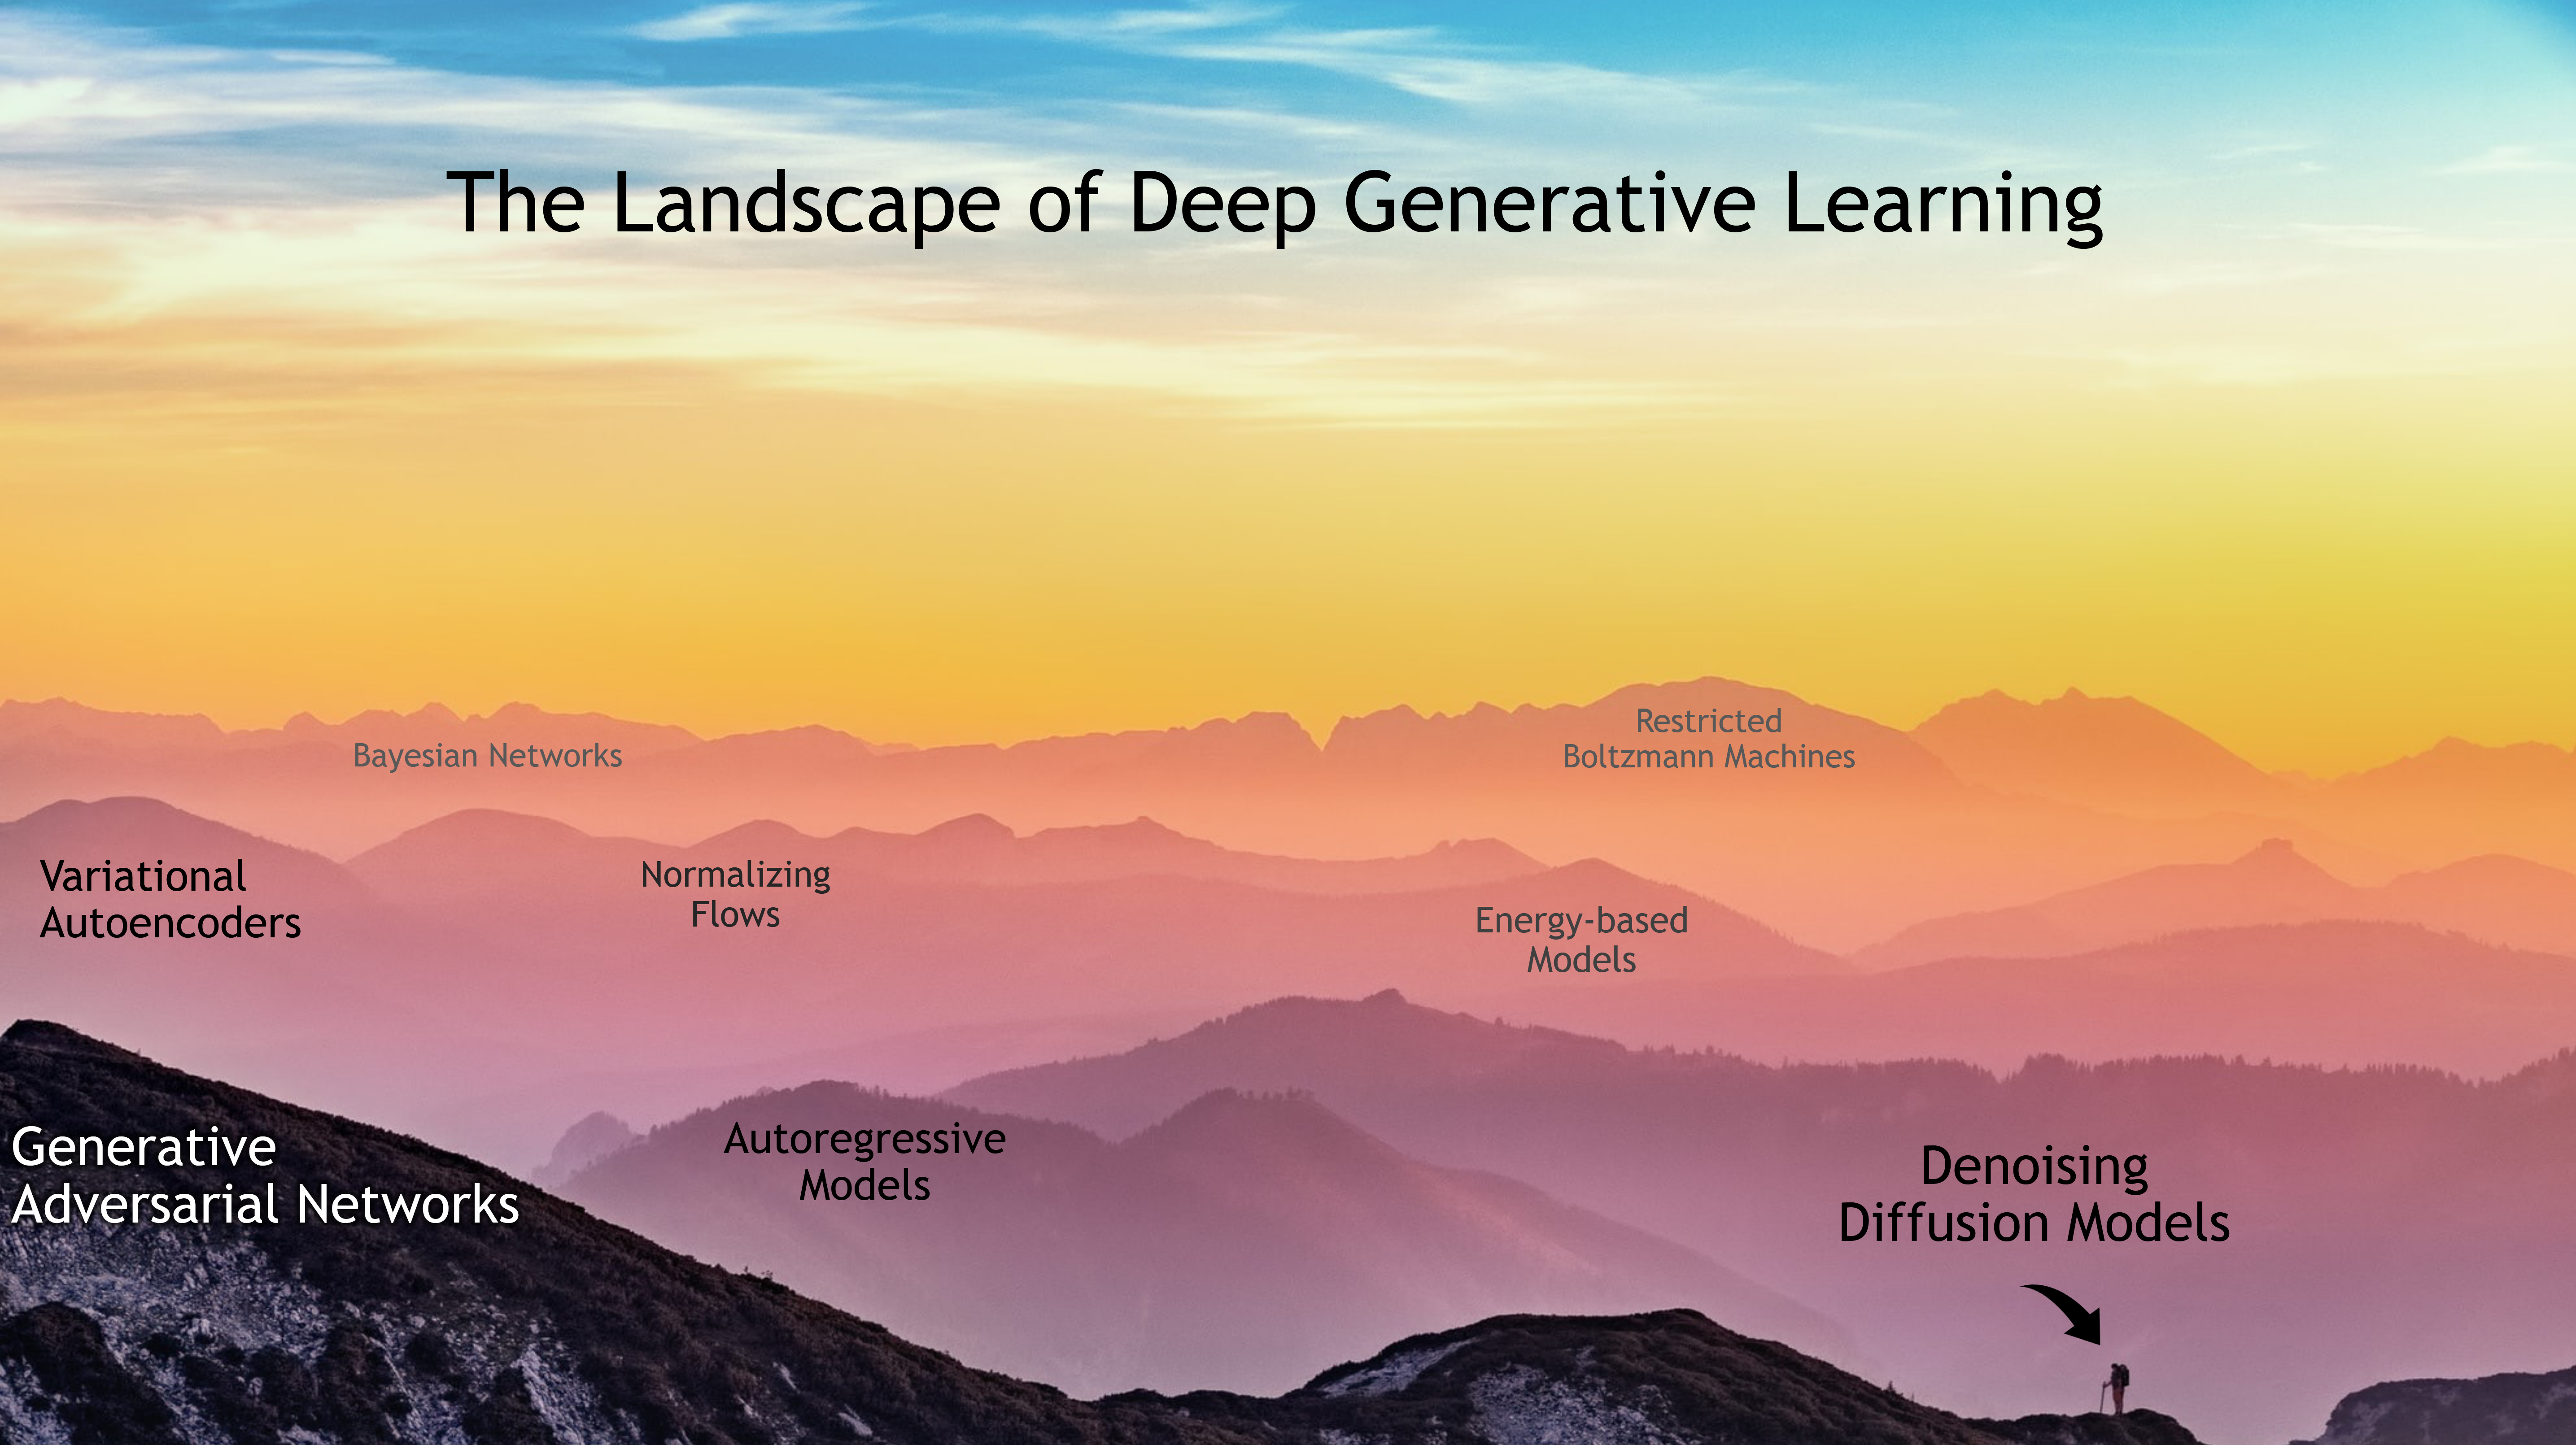
\includegraphics[width=0.9\linewidth]{figs/landscape.png}
%     \caption{\scriptsize 图像来源~\parencite{CVPR2023Tutorial}.}
%   \end{figure}
%   \bottomleftrefs
% \end{frame}
% \end{refsection}


\begin{refsection}
\begin{frame}{背景:扩散模型}

  \begin{figure}
    \begin{minipage}{0.95\linewidth}
      \footnotesize
      \textbf{去噪扩散模型包含两个过程:}
      \begin{itemize}
        \item 正向扩散过程:逐步向输入添加噪声。
        \item 反向去噪过程:通过去噪学习生成数据。
      \end{itemize}
    \end{minipage}
    \vspace{2em}

    \centering
    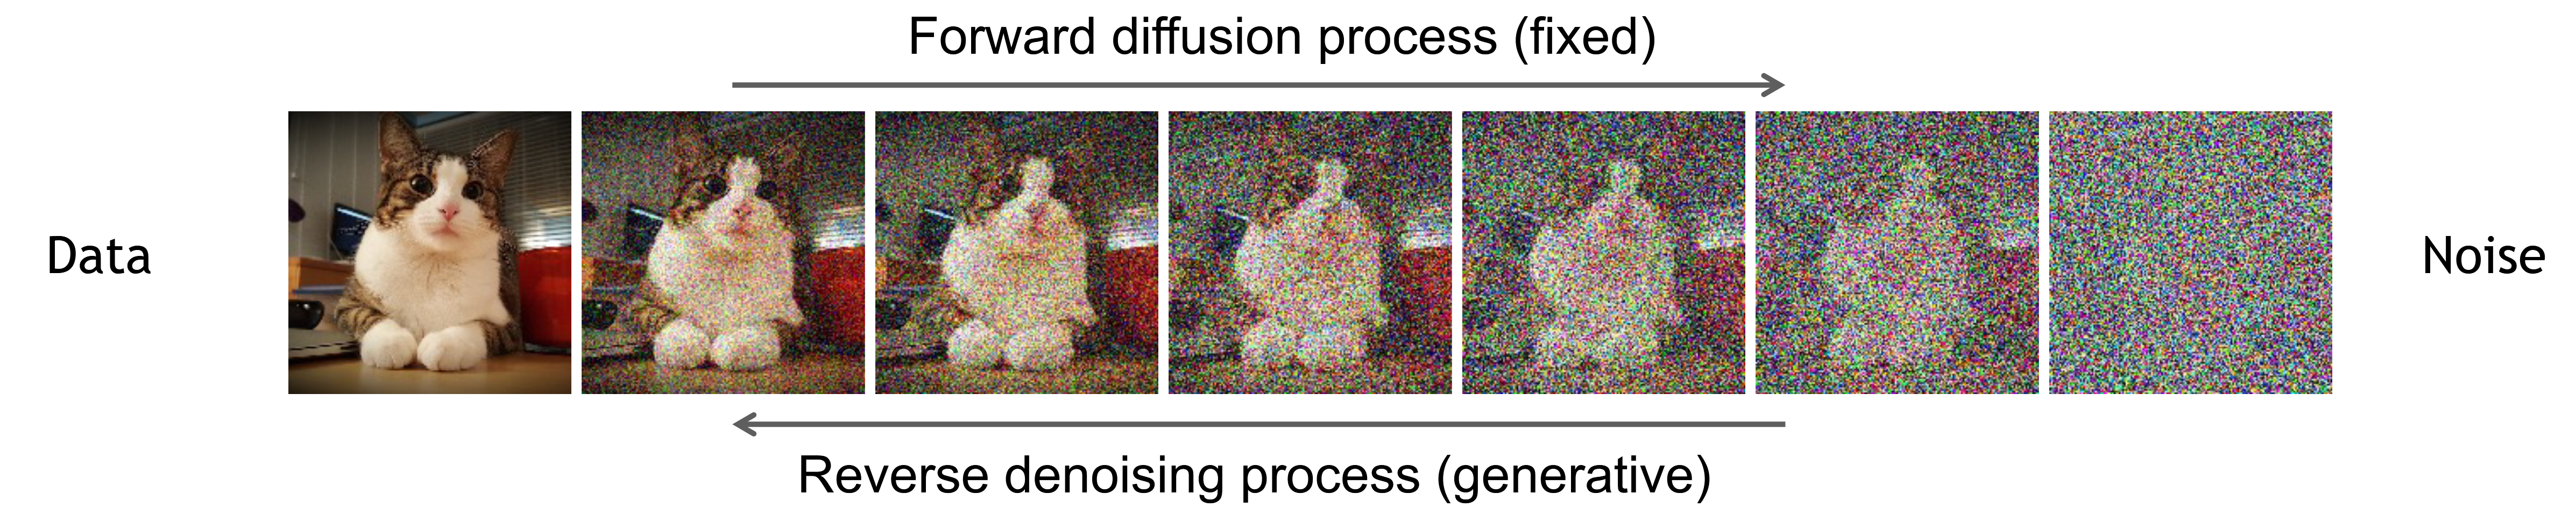
\includegraphics[width=1.0\linewidth]{figs/diffusion_high_level.png}

    \caption[]{\scriptsize 扩散模型通过迭代去噪生成数据~\parencite{sohl2015deep,ho2020denoising}.}
  \end{figure}

  \bottomleftrefs
\end{frame}
\end{refsection}

% --- 幻灯片4:扩散模型基础 ---
% \begin{refsection}
% \begin{frame}{扩散模型:正向与反向过程}
%   \footnotesize
%   \textbf{正向(扩散)过程:}
%   \begin{align*}
%     q(\mathbf{x}_t \mid \mathbf{x}_{t-1}) &= \mathcal{N}(\mathbf{x}_t; \sqrt{1-\beta_t}\,\mathbf{x}_{t-1}, \beta_t \mathbf{I}) \\
%     q(\mathbf{x}_{1:T} \mid \mathbf{x}_0) &= \prod_{t=1}^T q(\mathbf{x}_t \mid \mathbf{x}_{t-1}) \\
%     &\text{等价于} 
%     \mathbf{x}_t = \sqrt{\bar{\alpha}_t}\,\mathbf{x}_0 + \sqrt{1-\bar{\alpha}_t}\,\boldsymbol{\epsilon}, \quad \boldsymbol{\epsilon} \sim \mathcal{N}(\mathbf{0}, \mathbf{I})
%   \end{align*}

%   \footnotesize
%   \textbf{反向(去噪)过程:}
%   \begin{align*}
%     p_\theta(\mathbf{x}_{t-1} \mid \mathbf{x}_t) &= \mathcal{N}(\mathbf{x}_{t-1}; \boldsymbol{\mu}_\theta(\mathbf{x}_t, t), \Sigma_\theta(\mathbf{x}_t, t)) \\
%     p_\theta(\mathbf{x}_{0:T}) &= p(\mathbf{x}_T) \prod_{t=1}^T p_\theta(\mathbf{x}_{t-1} \mid \mathbf{x}_t)
%   \end{align*}
%   \scriptsize
%   其中 $\mathbf{x}_0$ 为数据,$\beta_t$ 为噪声调度,$\bar{\alpha}_t = \prod_{s=1}^t (1-\beta_s)$。$p(\mathbf{x}_T) = \mathcal{N}(\mathbf{0}, \mathbf{I})$。

%   \scriptsize
%   \textbf{扩散模型通过学习逆转逐步加噪过程来生成数据。}~\parencite{sohl2015deep,ho2020denoising}
%   \bottomleftrefs
% \end{frame}
% \end{refsection}

% \begin{refsection}
% \begin{frame}{扩散模型:训练与推理}
%   \footnotesize
%   \textbf{训练目标:}
%   \begin{align*}
%     \mathcal{L}_{\mathrm{simple}} = \mathbb{E}_{\mathbf{x}_0, \boldsymbol{\epsilon}, t} \left[ \left\| \boldsymbol{\epsilon} - \boldsymbol{\epsilon}_\theta(\sqrt{\bar{\alpha}_t}\mathbf{x}_0 + \sqrt{1-\bar{\alpha}_t}\boldsymbol{\epsilon}, t) \right\|^2 \right]
%   \end{align*}
%   其中 $\boldsymbol{\epsilon} \sim \mathcal{N}(\mathbf{0}, \mathbf{I})$,$\bar{\alpha}_t = \prod_{s=1}^t (1-\beta_s)$。

%   \vspace{0.5em}
%   \textbf{推理(采样):}
%   \begin{itemize}
%     \item 从纯噪声开始:$\mathbf{x}_T \sim \mathcal{N}(\mathbf{0}, \mathbf{I})$
%     \item 对 $t = T, \ldots, 1$:
%       \begin{itemize}
%         \item 预测噪声:$\boldsymbol{\epsilon}_\theta(\mathbf{x}_t, t)$
%         \item 计算均值:$\boldsymbol{\mu}_\theta(\mathbf{x}_t, t)$
%         \item 采样:$\mathbf{x}_{t-1} \sim \mathcal{N}(\boldsymbol{\mu}_\theta(\mathbf{x}_t, t), \Sigma_\theta(\mathbf{x}_t, t))$
%       \end{itemize}
%     \item 重复直到得到 $\mathbf{x}_0$(生成样本)
%   \end{itemize}

%   \vspace{0.5em}
%   \scriptsize
%   \textbf{训练:} 最小化简化目标~\parencite{ho2020denoising}.\\
%   \textbf{推理:} 通过迭代去噪从随机噪声生成数据。
%   \bottomleftrefs
% \end{frame}
% \end{refsection}

%--- 幻灯片5:遥感图像生成中的应用:DiffusionSat、CRS-Diff、Text2Earth ---

\begin{refsection}
  \begin{frame}{遥感图像生成应用:Text2Earth}
    \begin{figure}
      \centering
      \includegraphics[width=0.9\linewidth]{figs/text2earth.png}
      \caption[]{\scriptsize Text2Earth:面向文本驱动地球观测的基础模型~\parencite{text2earth2025}.}
    \end{figure}
    \bottomleftrefs
  \end{frame}
\end{refsection}

\begin{refsection}
  \begin{frame}{Text2Earth:示例结果}
    \begin{figure}
      \centering
      \includegraphics[width=0.9\linewidth]{figs/text2earth_results.png}
      \caption[]{\scriptsize Text2Earth 生成的示例结果~\parencite{text2earth2025}.}
    \end{figure}
    \bottomleftrefs
  \end{frame}
\end{refsection}

\begin{refsection}
\begin{frame}{遥感图像生成应用:CRS-Diff}
  \begin{figure}
    \centering
    \includegraphics[width=0.9\linewidth]{figs/crsdiff.png}
    \caption[]{\scriptsize CRS-Diff:可控遥感图像生成框架~\parencite{tang2024crsdiff}.}
  \end{figure}
  \bottomleftrefs
\end{frame}
\end{refsection}

\begin{refsection}
\begin{frame}{CRS-Diff:示例结果}
  \begin{figure}
    \centering
    \includegraphics[width=0.9\linewidth]{figs/crsdiff_results.png}
    \caption[]{\scriptsize CRS-Diff 生成的示例结果~\parencite{tang2024crsdiff}.}
  \end{figure}
  \bottomleftrefs
\end{frame}
\end{refsection}


%--- 幻灯片6a:DiffusionSat 框架 ---
\begin{refsection}
\begin{frame}{DiffusionSat:框架概览}
  \begin{figure}
    \centering
    \includegraphics[width=0.9\linewidth]{figs/diffusionsat.png}
    \caption[]{\scriptsize DiffusionSat:面向卫星影像的生成式基础模型~\parencite{diffusionset2024}.}
  \end{figure}
  \bottomleftrefs
\end{frame}
\end{refsection}

%--- 幻灯片6b:DiffusionSat 超分辨率 ---
% \begin{refsection}
% \begin{frame}{DiffusionSat:超分辨率结果}
%   \begin{figure}
%     \centering
%     \includegraphics[width=0.9\linewidth]{figs/diffusionsat_sr_results.png}
%     \caption[]{\scriptsize DiffusionSat 多光谱超分辨率示例结果~\parencite{diffusionset2024}.}
%   \end{figure}
%   \bottomleftrefs
% \end{frame}
% \end{refsection}

%--- 幻灯片6c:DiffusionSat 图像修复 ---
% \begin{refsection}
% \begin{frame}{DiffusionSat:图像修复结果}
%   \begin{figure}
%     \centering
%     \includegraphics[width=0.9\linewidth]{figs/diffusionsat_inpainting_results.png}
%     \caption[]{\scriptsize DiffusionSat 用于遥感图像修复的示例结果~\parencite{diffusionset2024}.}
%   \end{figure}
%   \bottomleftrefs
% \end{frame}
% \end{refsection}



%--- 幻灯片8:Q&A ---
\begin{refsection}
\begin{frame}[plain]
  \vfill
  \centering
  {\LARGE \textbf{问答环节}}
  \vfill
\end{frame}
\end{refsection}

\begin{refsection}
  \begin{frame}{项目作业:研究主题}
    \textbf{核心问题:} \\
    \vspace{0.5em}
    生成模型合成数据是否已准备好用于图像识别?
  
    \vspace{1em}
    \begin{itemize}
      \item 生成模型合成数据是当前流行的数据增强新方式~\parencite{heSYNTHETICDATAGENERATIVE2022,tokerSatSynthAugmentingImageMask2024}.
      \item 本项目将探索此类增强是否有助于遥感领域的下游任务,如文本-图像检索、图像场景分类和超分辨率等。
      % \item 分析最新研究并进行自己的实验。
    \end{itemize}
    \bottomleftrefs
  \end{frame}
  \end{refsection}

  
\begin{refsection}
  \begin{frame}{背景:为什么要用合成数据?}
    \begin{itemize}
      \item 手工数据采集与标注成本高、耗时长。
      \item 生成模型合成数据可实现大规模数据增强。
      \item 合成数据对遥感下游任务的有效性仍在积极研究中。
    \end{itemize}
    \begin{minipage}{0.5\linewidth}
      \includegraphics[width=\linewidth]{figs/Visualization_of_different_strategies_of_synthetic_data_in_zeroshot_settings.png}
    \end{minipage}%
    \hfill
    \begin{minipage}{0.4\linewidth}
      \vspace{0.5em}
      {\scriptsize
      \textbf{零样本设置下不同合成数据策略的可视化~\parencite{heSYNTHETICDATAGENERATIVE2022}.} 展示了真实数据与不同策略(基础B、语言增强LE、语言增强+CLIP过滤LE+CF)合成图像的可视化对比。
      }
    \end{minipage}
    \bottomleftrefs
  \end{frame}
  \end{refsection}
  
  
  
  \begin{refsection}
    \begin{frame}{实验设置:下游任务的生成式数据}
      \begin{itemize}
        \item 我们利用最先进的生成模型(如 \textbf{DiffusionSat}~\parencite{diffusionset2024} 和 \textbf{Text2Earth}~\parencite{text2earth2025})进行合成数据增强。
        \item \textbf{两种主要策略:}
        \begin{enumerate}
          \item \textbf{文本到图像生成:}
            \begin{itemize}
              \item 生成文本-图像对。
              \item 支持图像场景分类、图文检索等任务。
            \end{itemize}
          \item \textbf{超分辨率生成:}
            \begin{itemize}
              \item 生成低分辨率(LR)与高分辨率(HR)配对图像。
              \item 支持遥感超分辨率任务。
            \end{itemize}
        \end{enumerate}
      \end{itemize}
      \vspace{1em}
      % \begin{figure}
      %   \centering
      %   \fbox{\rule{0pt}{2in} \rule{0.8\linewidth}{0pt}} % Empty figure placeholder
      %   \caption{\scriptsize 实验流程:为遥感下游任务生成合成数据。}
      % \end{figure}
      \bottomleftrefs
    \end{frame}
    \end{refsection}

    %--- 附加幻灯片:项目作业下游任务 ---

% \begin{refsection}
%   \begin{frame}{下游任务概览}
%     \begin{itemize}
%       \item 本项目关注两个关键下游任务:
%       \begin{enumerate}
%         \item \textbf{图像场景分类}(如CLIP等基础模型)
%         \item \textbf{图像超分辨率}(如Real-ESRGAN等生成模型)
%       \end{enumerate}
%       \item 我们旨在评估合成数据是否提升这些任务的模型表现。
%     \end{itemize}
%   \end{frame}
%   \end{refsection}
  
  \begin{refsection}
  \begin{frame}{CLIP 场景分类}
    % \textbf{CLIP: 对比式语言-图像预训练}
    \begin{figure}
      \centering
      \includegraphics[width=\linewidth]{figs/clip.png}
      \caption{\scriptsize CLIP~\parencite{radfordLearningTransferableVisual2021} 模型概览:图像与文本编码器联合训练,实现跨模态理解。}
    \end{figure}

    \bottomleftrefs
  \end{frame}
  \end{refsection}
  
  \begin{refsection}
  \begin{frame}{Real-ESRGAN 超分辨率}
    % \textbf{Real-ESRGAN: 增强型超分辨率生成对抗网络}
    \begin{figure}
      \centering
      \includegraphics[width=\linewidth]{figs/realesrgan.png}
      \caption{\scriptsize Real-ESRGAN~\parencite{wangRealESRGANTrainingRealWorld2021b} 框架:面向真实世界图像超分辨率的架构。}
    \end{figure}
    \bottomleftrefs
  \end{frame}
  \end{refsection}

  
\begin{refsection}
  \begin{frame}{场景分类与超分辨率基线模型}
    \textbf{场景图像分类:}
    \begin{itemize}
      \item \textbf{CLIP}~\parencite{radfordLearningTransferableVisual2021}
      \item \textbf{RemoteCLIP}~\parencite{liuRemoteCLIPVisionLanguage2024}
      \item \textbf{Git-RSCLIP}~\parencite{text2earth2025}
    \end{itemize}
    \textbf{超分辨率:}
    \begin{itemize}
      \item \textbf{Real-ESRGAN}~\parencite{wangRealESRGANTrainingRealWorld2021b}
      \item \textbf{StableSR}~\parencite{wangExploitingDiffusionPrior2024}
      \item \textbf{FaithDiff}~\parencite{chenFaithDiffUnleashingDiffusion2024}
      \item \textbf{EResShift}~\parencite{yueEfficientDiffusionModel2025}
    \end{itemize}
    % \begin{figure}
    %   \centering
    %   \includegraphics[width=0.7\linewidth]{figs/realesrgan.png}
    %   \caption{\scriptsize Real-ESRGAN 框架。}
    % \end{figure}
    \bottomleftrefs
  \end{frame}
  \end{refsection}

  %--- 幻灯片:下游任务数据集 ---
\begin{refsection}
  \begin{frame}{下游任务数据集}
    \textbf{文本到图像生成:}
    \begin{itemize}
      \item \textbf{RSICD}~\parencite{lu2017exploring}:遥感图像描述数据集,含10,921张图像,每张配有5条描述。
      \item \textbf{RSICap}~\parencite{hu2023rsgpt}:高质量数据集,包含2,585个人工标注的图文对。
      \item \textbf{UCM-Captions}~\parencite{qu2016deep}:源自UC Merced土地利用数据集,含2,100张图像,每张配有5条描述。
    \end{itemize}
    \vspace{1em}
    \textbf{超分辨率:}
    \begin{itemize}
      \item \textbf{fMoW}:Sentinel-2(10m GSD)~\parencite{congFunctionalMapWorld2022} 与 fMoW-RGB(0.3m)~\parencite{christieFunctionalMapWorld2018} 配对数据集。
    \end{itemize}
    \bottomleftrefs
  \end{frame}
  \end{refsection}

  
\begin{refsection}
  \begin{frame}{可能的结果}
    \begin{itemize}
      \item ~\parencite{heSYNTHETICDATAGENERATIVE2022} 的结果表明,合成数据增强在遥感基准上带来了显著的准确率提升。
    \end{itemize}
    \begin{figure}
      \centering
      \includegraphics[width=0.70\linewidth]{figs/syn_aug_results.png}
      \caption{\scriptsize 使用合成数据增强后分类性能提升~\parencite{heSYNTHETICDATAGENERATIVE2022}.}
    \end{figure}
    \bottomleftrefs
  \end{frame}
  \end{refsection}

  \begin{refsection}
    \begin{frame}{基于扩散的合成数据增强更优}
      \begin{figure}
        \centering
        \includegraphics[width=0.7\linewidth]{figs/satsynth_comparison.png}
        \caption{\scriptsize SatSynth 表格:基于扩散的合成数据增强在分割精度上优于传统增强方法~\parencite{tokerSatSynthAugmentingImageMask2024}.}
      \end{figure}
      \vspace{-2.5em}
      \begin{table}[]
        \centering
        \caption[]{\scriptsize 定量对比:iSAID~\parencite{waqas2019isaid} 数据集上的平均IoU。}
        \scriptsize
        \setlength{\tabcolsep}{2.5pt}
        \begin{tabular}{@{}l|cccc@{}}
        \toprule
        \textbf{无增强} & \textbf{本方法} & \textbf{Cutout~\parencite{devriesImprovedRegularizationConvolutional2017}} & \textbf{CutMix~\parencite{yunCutmixRegularizationStrategy2019}} & \textbf{Copy-Paste~\parencite{ghiasiSimpleCopyPasteStrong2021}} \\
        \midrule
        50.25 & \textbf{51.11} & 50.47 & 50.60 & 50.51 \\
        \bottomrule
        \end{tabular}
      \end{table}
    
      \bottomleftrefs
    \end{frame}
    \end{refsection}
    
% \begin{frame}[allowframebreaks]{参考文献}
%   \printbibliography
% \end{frame}